%!TEX ROOT = thesis.tex
\chapter{Introduction, Background Story, Motivations}
\section{First Test and I need a really long title, please do oblige me won't you? Just a few more words and yes we're there}
\lipsum[1-2]

\begin{figure}[hbt!]\centering
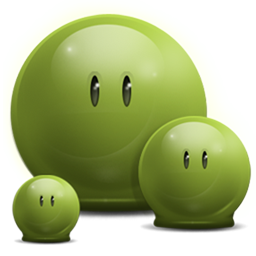
\includegraphics[width=.3\textwidth]{green}
\caption{First figure. OK?}
\end{figure}

\subsection{Second Test}
Their \cite{audibert:2004} requirements\footnote{See here, how weird, how to fill out an entire line. See here, how weird, how to fill out an entire line. See here, how weird, how to fill out an entire line. See here, how weird, how to fill out an entire line. See here, how weird, how to fill out an entire line. } are really amazing\footnote{don't you agree?} \cite{budanitsky:hirst:2006}.

\begin{figure}[hbt!]\centering
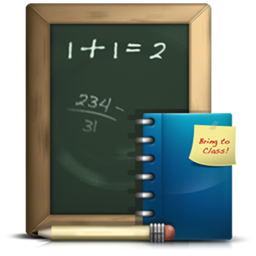
\includegraphics[width=.3\textwidth]{school}
\caption{Second figure. Now I need a long caption to test out how things look in the List of Figures. Is this long enough yet? Is it? Is it?}
\end{figure}

How how?

\subsubsection{This works?}
Does it?\index{test} Great. Let's talk about \glspl{LI} and \glspl{POS} in \gls{NLP}. I mention again \glspl{LI}. Oh I have a symbol too, it's \gls{theta}.

\section{Yeah}
\lipsum[5]

\begin{table}[hbt!]
\caption{This is a table}
\centering
\begin{tabular}{ l c r }
\hline
Hey & How's it & Going?\\ \hline
Fine! & Just great. & See ya!\\
Fine! & Just great. & See ya!\\
\hline
\end{tabular}
\end{table}

\lipsum[7-12]